\documentclass[hyperref=unicode,graphics=pdflatex,13pt,xcolor={usenames,dvipsnames}]{beamer}


\usepackage[usenames,dvipsnames]{xcolor}
\usepackage[noend]{algorithmic}
\usepackage{algorithm}
\usepackage{xspace}
\usepackage[algo2e,ruled,vlined,linesnumbered]{algorithm2e}
\let\oldnl\nl% Store \nl in \oldnl
\newcommand{\nonl}{\renewcommand{\nl}{\let\nl\oldnl}}% Remove line number for one line

\usepackage{amsmath}
\usepackage{mathtools}
\usepackage{cite}
\usepackage{array}
\usepackage{multirow}
\usepackage{tabularx}
\usepackage{wasysym} %smiles

\usepackage{pgfplots}
\usepgfplotslibrary{statistics}
\usetikzlibrary{decorations.pathreplacing,calc,tikzmark, patterns,arrows.meta}




\mode<presentation>
{
  % \usetheme{Goettingen}
%  \usecolortheme{crane}
  \setbeamercovered{invisible}
%  \useoutertheme{infolines}
%  \setbeamertemplate{headline}{} % removes the headline that infolines inserts
}

\graphicspath{{../pic/},{pic/}}

\setbeamertemplate{frametitle continuation}{(\insertcontinuationcount)}
\setbeamertemplate{footline}[text line]
{
  % \leavevmode%
  \hbox{%
    % \hspace{3mm}
    \begin{beamercolorbox}[ht=2.25ex,dp=1ex,left,wd=0.18\textwidth]{author in head/foot}%
        \usebeamerfont{author in head/foot}
        \insertshortauthor
    \end{beamercolorbox}%    
    \begin{beamercolorbox}[ht=2.25ex,dp=1ex,left,wd=0.63\textwidth]{title in head/foot}%
        \usebeamerfont{title in head/foot}
        \insertshorttitle
    \end{beamercolorbox}%
    \begin{beamercolorbox}[ht=2.25ex,dp=1ex,right,wd=0.2\textwidth]{framenumber}%
        \insertframenumber{}
        \hspace*{2ex} 
    \end{beamercolorbox}
  }%
}
\setbeamertemplate{navigation symbols}{}
\setbeamertemplate{itemize/enumerate body begin}{\normalsize}
\setbeamertemplate{itemize/enumerate subbody begin}{\normalsize}
\setbeamersize{text margin left=5mm,text margin right=5mm} 
% \setbeamerfont{page number in head/foot}{size=\large}
% \beamertemplatenavigationsymbolsempty
\usefonttheme[onlymath]{serif}

\usepackage[utf8]{inputenc}
\usepackage[T2A]{fontenc}
\usepackage[russian]{babel}
\usepackage{colortbl}
\usepackage{multirow}

\usepackage{algorithm}
\usepackage{algorithmic}

\renewcommand\emph[1]{{\color{blue}{#1}}}
\newcommand\blue[1]{{\color{blue}{#1}}}
\newcommand\red[1]{{\color{red}{#1}}}
\newcommand\green[1]{{\color{green!50!darkgray}{#1}}}
\newcommand\pitem{\pause\item}

\newcommand\N{\mathbb{N}}
\newcommand\R{\mathbb{R}}

\DeclareMathOperator{\Bin}{Bin}
\DeclareMathOperator{\Geom}{Geom}
\DeclareMathOperator{\pow}{pow}
\DeclareMathOperator{\Bern}{Bern}
\DeclareMathOperator{\Var}{Var}

\deftranslation[to=russian]{Theorem}{Теорема}

\title[Дискретные случайные величины]{Дискретные случайные величины}

\author[Антипов Д. С.]
{Антипов Денис Сергеевич}
\institute{
Университет ИТМО, Санкт-Петербург, Россия\\
~\\
}
\date[]{
\includegraphics[height=2cm]{itmo-white-rus.png} \\
18 февраля 2021 г.}


\begin{document}

\begin{frame}[noframenumbering,plain]
%   \advance\textwidth2cm
% \hsize\textwidth
% \columnwidth\textwidth
  \titlepage
\end{frame}

\section{Случайная величина}
\begin{frame}
  \frametitle{Случайная величина}

  Случайная величина (с.в.) --- \emph{функционал}, заданный на $\Omega$.

  \[
    X: \Omega \to \R
  \]
  \pause
  \begin{itemize}
    \pitem \emph{NB:} этот функционал должен быть \emph{измерим} по используемой мере $\Pr$ 
  \end{itemize}

  \pause
  \vspace{1em}
  Договоримся об обозначениях

  \begin{itemize}
    \item Большая буква ($X$, $Y$, $Z$, etc) --- случайная величина (как \emph{отображение})
    \item Маленькая буква ($x$, $y$, $z$, etc) --- значение случайной величины (\emph{число})
  \end{itemize}
\end{frame}

\begin{frame}
  \frametitle{Примеры случайных величин}
  На конечной $\Omega$

  \begin{itemize}
    \item Бросок кости: $X$ --- число на верхней грани
    \begin{itemize}
      \item \{
\includegraphics[height=0.8em]{d6-1.png} $\to 1$, 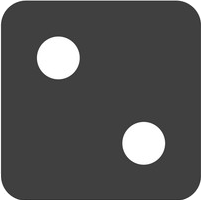
\includegraphics[height=0.8em]{d6-2.png} $\to 2$, 
\includegraphics[height=0.8em]{d6-3.png} $\to 3$, 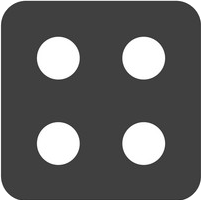
\includegraphics[height=0.8em]{d6-4.png} $\to 4$, 
\includegraphics[height=0.8em]{d6-5.png} $\to 5$, 
\includegraphics[height=0.8em]{d6-6.png} $\to 6$\}
    \end{itemize}
    \item Хоккейный матч: $X$ --- очки домашней команды
    \begin{itemize}
      \item \{В $\to 2$, ВО $\to 2$, ВБ $\to 2$, ПБ $\to 1$, ПО $\to 1$, П $\to 0$\}
    \end{itemize} 
  \end{itemize}

  \pause
  На счетной $\Omega$
  \begin{itemize}
    \item Бросаем монету до первого орла: $X$ --- число бросков
  \end{itemize}

  \pause
  На несчетной $\Omega$
  \begin{itemize}
    \item Бросаем дротик в мишень для дартса: $X$ --- очки согласно правилам игры
    \item Крутим волчок в ЧГК: $X$ --- угол, на котором он остановится
    \begin{itemize}
      \item $Y$ --- население города, из которого пришел вопрос
      \item $Z$ --- вероятность того, что на выбранный вопрос знатоки ответят
    \end{itemize}
  \end{itemize}
\end{frame}

\begin{frame}
  \frametitle{Дискретные случайные величины}

  \emph{Дискретными} называются те с.в., которые определены на не более, чем счетной $\Omega$

  \vspace{1cm}\pause 
  \emph{NB:} Множеством знaчений дискретной с.в. может быть любое подмножество $\R$ (не более, чем счетное, разумеется)

  \vspace{1cm}\pause
  \emph{NB-2:} Никаких проблем с измеримостью дискретной с.в. как функции обычно нет, поэтому этот вопрос мы будем опускать
\end{frame}

\section{Функция вероятностей}
\begin{frame}
  \frametitle{Функция вероятности}

  Можно рассматривать $(X = x)$ как \emph{событие}, так как оно задает какое-то множество исходов из $\Omega$. Тогда у этого события должна быть \emph{вероятность}.
  
  \pause

  \begin{center}
    \begin{tikzpicture}[rounded corners]
      \node [draw, rectangle, fill=blue!20, minimum height = 1.5cm, minimum width = 2.5cm] at (0,0) {$
      p_X(x) = \Pr(X = x) = \Pr(\{\omega \in \Omega \mid X(\omega) = x\})$};
    \end{tikzpicture}
  \end{center}

  $p_X$ называется \emph{функцией вероятности} с.в. $X$.

  \pause
  Ее свойства:
  \begin{itemize}
    \item $p_X(x) \ge 0$
    \item $\sum_x p_X(x) = 1$
  \end{itemize}
\end{frame}

\section{Известные распределения}
\begin{frame}
  \frametitle{Примеры случайных величин}
  Если нам дано какое-то \emph{распределение} $\mathcal{D}$ и с.в. $X$ ему следует, мы пишем $X \sim \mathcal{D}$ 

  Примеры распределений (законов):
  \begin{itemize}
    \item Бернулли
    \item Равномерное
    \item Биномиальное
    \item Геометрическое
    \item Гипер-геометрическое
    \item Степенное
  \end{itemize}
\end{frame}

\begin{frame}
  \frametitle{Распределение Бернулли}
  \begin{align*}
    X \sim \Bern(p) \Leftrightarrow \begin{cases}
      p_X(0) = (1 - p), \\
      p_X(1) = p, \\
      p_X(x) = 0 \text{ для всех остальных } x. 
    \end{cases}
  \end{align*}

  \pause
  \begin{itemize}
    \item $p$ --- параметр распределения, вероятность \emph{успеха}
    \item С.в. $X$ может быть индикатором события $A$:
    \begin{itemize}
      \item $\omega \in A \Rightarrow X(\omega) = 1$
      \item $\omega \notin A \Rightarrow X(\omega) = 0$
    \end{itemize}
  \end{itemize}
    \begin{center}
      \scalebox{0.5}{
        \begin{tikzpicture}
          \begin{axis}[ybar, ymin=0, ymax=1,
            ytick={0, 0.3, 0.7, 1},
            yticklabels={0, $p$, $(1 - p)$, 1},
            grid=major,
            ylabel={$p_X(x)$},
            xlabel={$x$}]
            \addplot
            [draw=blue, fill=blue] 
            coordinates
              {(0, 0.7) (1,0.3)};
          \end{axis}
        \end{tikzpicture}
      }
    \end{center}
\end{frame}


\begin{frame}
  \frametitle{Равномерное дискретное распределение}

  \begin{center}
    \scalebox{0.5}{
      \begin{tikzpicture}
        \begin{axis}[ybar, ymin=0, ymax=1,
          ytick={0, 0.2, 1},
          yticklabels={0, $\frac{1}{b - a + 1}$, 1},
          xtick=data,
          xticklabels={$a$, $a + 1$, $\cdots$, $b - 1$, $b$},
          grid=major,
          ylabel={$p_X(x)$},
          xlabel={$x$}]
          \addplot
          [draw=blue, fill=blue] 
          coordinates
            {(0, 0.2) (1,0.2) (2,0.2) (3,0.2) (4,0.2)};
        \end{axis}
      \end{tikzpicture}
    }
  \end{center}

  \vspace{-0.5cm}
  \begin{align*}
    X \sim U(a, b) = \begin{cases}
      p_X(x) = \frac{1}{b - a + 1}, &\text{ если } x \in [a..b], \\
      p_X(x) = 0, &\text{ иначе.}
    \end{cases}
  \end{align*}

  \begin{itemize}
    \item $a$, $b$ --- целочисленные параметры ($a \le b$)
    \item $\Omega = [a..b]$
    \item $X(\omega) = \omega$ 
  \end{itemize}

\end{frame}

\begin{frame}
  \frametitle{Биномиальное распределение}
  Проведем $n$ независимых опытов по схеме Бернулли с вероятностью успеха $p$. $X$ --- \emph{число успехов}.

  \begin{align*}
    X \sim \Bin(n, p) \Leftrightarrow X = \sum_{i = 1}^n X_i,
  \end{align*}
  где все $X_i \sim \Bern(p)$.
  
  \pause

  \begin{center}
    \begin{tikzpicture}[rounded corners]
      \node [draw, rectangle, fill=blue!20, minimum height = 1.5cm, minimum width = 4.5cm] at (0,0) {};
      \node at (-1.3, 0) {$p_X(x) = ?$};
      \onslide<4->{
        \fill [blue!20] (-0.7, -0.3) rectangle (1, 0.3);
        \node at (0.7, 0) {$\binom{n}{x}p^x(1 - p)^{n - x}$};
      }
    \end{tikzpicture}
  \end{center}

  \pause
  \begin{itemize}
    \item Вероятность конкретного исхода, в котором ровно $x$ успехов:
    \begin{align*}
      \Pr(\omega) = p^x (1 - p)^{n - x}
    \end{align*}
    \item Всего таких исходов $\binom{n}{x}$ 
  \end{itemize}
\end{frame}

\begin{frame}
  \frametitle{Функции вероятностей биномиального распределения}

  \begin{center}
    \scalebox{0.45}{
      \begin{tikzpicture}[declare function={binom(\k,\n,\p)=\n!/(\k!*(\n-\k)!)*\p^\k*(1-\p)^(\n-\k);}]
        \begin{axis}[name=a1, ybar, title={$n = 5$}, samples at={0,...,5}, ylabel={$p_X(x), p = 0.5$}, xlabel={$x$}]
          \addplot[draw=blue, fill=blue]  {binom(x,5,0.5)};
        \end{axis}
        \begin{axis}[name=a2, at={ (a1.south east) }, xshift=2cm, ybar, bar width = 5pt, title={$n = 20$}, samples at={0,...,20}, xlabel={$x$}]
          \addplot[draw=blue, fill=blue]  {binom(x,20,0.5)};
        \end{axis}
        \begin{axis}[at={ (a2.south east) }, xshift=2cm, ybar, bar width = 2pt, title={$n = 100$}, samples at={0,...,100}, xlabel={$x$}]
          \addplot[draw=blue, fill=blue]  {binom(x,100,0.5)};
        \end{axis}
      \end{tikzpicture}
    }

    \scalebox{0.45}{    
    \begin{tikzpicture}[declare function={binom(\k,\n,\p)=\n!/(\k!*(\n-\k)!)*\p^\k*(1-\p)^(\n-\k);}]
      \begin{axis}[name=a1, ybar, samples at={0,...,5}, ylabel={$p_X(x), p = 0.2$}, xlabel={$x$}]
        \addplot[draw=blue, fill=blue]  {binom(x,5,0.2)};
      \end{axis}
      \begin{axis}[name=a2, at={ (a1.south east) }, xshift=2cm, ybar, bar width = 5pt, samples at={0,...,20}, xlabel={$x$}]
        \addplot[draw=blue, fill=blue]  {binom(x,20,0.2)};
      \end{axis}
      \begin{axis}[at={ (a2.south east) }, xshift=2cm, ybar, bar width = 2pt, samples at={0,...,100}, xlabel={$x$}]
        \addplot[draw=blue, fill=blue]  {binom(x,100,0.2)};
      \end{axis}
    \end{tikzpicture}
    }
  \end{center}

  \emph{NB:} везде разные масштабы оси $OY$
\end{frame}

\begin{frame}
  \frametitle{Геометрическое распределение}
  Проводим независимые эксперименты по схеме Бернулли с вероятностью успеха $p$ до первого успешного исхода. $X$ --- \emph{число экспериментов}, которые мы проводим.

  \begin{align*}
    X \sim Geom(p) \Leftrightarrow X = \min\{i \in \N \mid X_i = 1\},
  \end{align*}
  где $X_i \sim \Bern(p)$.
  
  \pause

  \begin{center}
    \begin{tikzpicture}[rounded corners]
      \node [draw, rectangle, fill=blue!20, minimum height = 1.5cm, minimum width = 4.5cm] at (0,0) {};
      \node at (-1.3, 0) {$p_X(x) = ?$};
      \onslide<3->{
        \fill [blue!20] (-0.7, -0.3) rectangle (1, 0.3);
        \node at (0.7, 0) {$p(1 - p)^{x - 1}$};
      }
    \end{tikzpicture}
  \end{center}

  \pause
  \begin{columns}
    \begin{column}{0.75\textwidth}
      \begin{itemize}
        \item Вероятность, что первые $x - 1$ неуспешны:
        \begin{align*}
          \Pr(X_1 = X_2 = \dots X_{x - 1} = 0) = (1 - p)^{x - 1}
        \end{align*}
        \item Вероятность, что $x$-ый исход успешен: 
        \begin{align*}
          \Pr(X_x = 1) = p 
        \end{align*}
      \end{itemize}
    \end{column}
    \begin{column}{0.25\textwidth}
      \scalebox{0.35}{
      \begin{tikzpicture}[declare function={geom(\k,\p)=\p*(1-\p)^(\k-1);}]
        \begin{axis}[ybar, ymin=0,
          % ytick=data,
          % yticklabels={0, $p$},
          grid=major,
          samples at={1,...,10}, ylabel={$p_X(x)$}, xlabel={$x$}]
          \addplot[draw=blue, fill=blue]  {geom(x,0.2)};
        \end{axis}
      \end{tikzpicture}
    }
    \end{column}
  \end{columns}
\end{frame}

\begin{frame}
  \frametitle{Уточнение}

  Есть исход, при котором $X = +\infty$, но его вероятность равна нулю.

  \begin{align*}
    \Pr(X = \infty) \le \Pr(X_1 = \dots = X_n = 0) = (1 - p)^n
  \end{align*}
  для любого $n$. Если допустить, что $\Pr(X = \infty) = q > 0$, то возьмем $n \ge \log_{1 - p} q$, получим, что вероятность подсобытия больше, чем вероятность события (\emph{Противоречие} со свойствами вероятностной меры).  
\end{frame}

\section{Матожидание}
\begin{frame}
  \frametitle{Математическое ожидание с.в.}

  Если много раз повторить один и тот же эксперимент, то каков будет средний результат?

  \begin{itemize}
    \item Бросаем честную кость d6. Что в среднем?
    \item $\frac{1}{6} \cdot 1 + \frac{1}{6} \cdot 2 + \frac{1}{6} \cdot 3 + \frac{1}{6} \cdot 4 + \frac{1}{6} \cdot 5 + \frac{1}{6} \cdot 6 = 3.5$
  \end{itemize}

  \pause

  \begin{center}
    \begin{tikzpicture}[rounded corners]
      \node [draw, rectangle, fill=blue!20, minimum height = 1.5cm, minimum width = 4.5cm] at (0,0) {
      \begin{minipage}{0.4\textwidth}
        $$E(X) = \sum_x x \cdot p_X(x)$$
      \end{minipage}};
    \end{tikzpicture}
  \end{center}

  \pause
  \emph{NB:} Матожидание определено только когда этот ряд \emph{абсолютно сходится}

  \pause
  \emph{NB-2:} Матожидание --- \emph{функционал} на множестве с.в.
\end{frame}

\begin{frame}
  \frametitle{Матожидание некоторых с.в.}

  $X \sim \Bern(p)$
  
  \begin{align*}
    E(X) = 0 \cdot (1 - p) + 1 \cdot p = p
  \end{align*}

  $X \sim U(a, b)$
  \begin{align*}
    E(X) = \sum_{i = a}^b \frac{i}{b - a + 1} = \frac{a + b}{2}
  \end{align*}  
\end{frame}

\begin{frame}
  \frametitle{Элементарные свойства матожидания}
  \begin{itemize}
    \item \emph{Неотрицательность:} $X \ge 0 \Rightarrow E(X) \ge 0$
    \item \emph{Ограниченность:} $X \in [a, b] \Rightarrow E(X) \in [a, b]$
    \item \emph{Матожидание константы:} $E(c) = c$
  \end{itemize}
\end{frame}

\begin{frame}
  \frametitle{Функции от с.в. и их матожидание}

  Пусть есть с.в. $X$ и функция $g: \R \to \R$. Тогда $Y = g(X)$ --- тоже с.в.

  \emph{Как посчитать $E(Y)$?}

  \begin{itemize}
    \pitem по определению: $E(Y) = \sum_y y p_Y(y)$
    \pitem 
      \begin{tikzpicture}[rounded corners]
        \node [draw, rectangle, fill=blue!20, minimum height = 1.5cm, minimum width = 4.5cm] at (0,0) {$E(Y) = \sum_x g(x)p_X(x)$};
      \end{tikzpicture}
  \end{itemize}
  
  \pause

  \begin{align*}
    \sum_x g(x)p_X(x) &= \sum_y \sum_{x: g(x) = y} g(x) p_X(x) \\
                      &= \sum_y y  \sum_{x: g(x) = y} p_X(x) = \sum_y y p_Y(y) = E(Y)
  \end{align*}


\end{frame}

\begin{frame}
  \frametitle{Линейность матожидания}
  \begin{center}
    \begin{tikzpicture}[rounded corners]
      \node [draw, rectangle, fill=blue!20, minimum height = 1cm, minimum width = 4.5cm] at (0,0) {
      \begin{minipage}{0.4\textwidth}
        $$E(aX + b) = aE(X) + b$$
      \end{minipage}};
    \end{tikzpicture}
  \end{center}

  \pause
  Позволяет легко пересчитывать матожидание с.в. не по определению.
  
  \begin{itemize}
    \item Пусть $X$ принимает четные значения от 0 до 100 с равной вероятностью.
    \item $X = 2Y$, где $Y \sim U(0, 50)$
    \item $E[X] = 2E[Y] = 50$
  \end{itemize}
  
  \pause \emph{NB:} Для всех линейных функций $g$ выполнено $E(g(X)) = g(E(X))$, но в общем случае это неверно

\end{frame}

\section{Дисперсия}
\begin{frame}
  \frametitle{Дисперсия}

  \onslide<3>{
    \begin{tikzpicture}[overlay]
      \node at (12, -4) {
\includegraphics[height=3cm]{harold.jpg}};   
    \end{tikzpicture}
  }

  \begin{columns}
    \begin{column}{0.7\textwidth}
      Иногда хотим оценить то, насколько с.в. \emph{отклоняется} от своего среднего значения $\mu$.

      \begin{itemize}
        \onslide<2->{
          \item Первая мысль: посчитать $E(X - \mu)$
        }
        \onslide<3->{
          \item $E(X - \mu)  = E(X) - \mu = 0$
        }
      \end{itemize}
    \end{column}
    \begin{column}{0.3\textwidth}
      \scalebox{0.4}{
        \begin{tikzpicture}[declare function={binom(\k,\n,\p)=\n!/(\k!*(\n-\k)!)*\p^\k*(1-\p)^(\n-\k);}]
          \begin{axis}[ybar, bar width = 5pt, samples at={0,...,20}, ylabel={$p_X(x)$}, xlabel={$x$}]
            \addplot[draw=blue, fill=blue]  {binom(x,20,0.2)};
          \end{axis}

          \node (exp) [red] at (1.7, -1) {$E(X) = \mu$}; 
          \draw [ultra thick, red] (exp) -- (1.7, 5.7);

          \draw [-{Triangle[width=18pt,length=8pt]}, red, line width=10pt] (1.8, 3) -- (4, 3) node [pos=1.0, right, red] {\Huge{?}};
          \draw [-{Triangle[width=18pt,length=8pt]}, red, line width=10pt] (1.6, 3) -- (0.5, 3);

        \end{tikzpicture}
      }
    \end{column}
  \end{columns}

  \pause\pause\pause

  \begin{center}
    \begin{tikzpicture}[rounded corners]
      \node [draw, rectangle, fill=blue!20, minimum height = 1cm, minimum width = 4.5cm] at (0,0) {$\Var(X) = E((X - \mu)^2)$};
    \end{tikzpicture}
  \end{center}

\end{frame}

\begin{frame}
  \frametitle{Несколько замечаний}

  \begin{center}
    \begin{tikzpicture}[rounded corners]
      \node [draw, rectangle, fill=blue!20, minimum height = 1cm, minimum width = 4.5cm] at (0,0) {$\Var(X) = E((X - \mu)^2)$};
    \end{tikzpicture}
  \end{center}

  \begin{itemize}
    \pitem Дисперсия считается как мотожидание \emph{функции от с.в.}
    \pitem Всегда \emph{неотрицательна}, равна нулю только у \emph{детерминированной} с.в.
    \pitem Почему не посчитать $|X - \mu|$? Просто так удобнее. Чем --- узнаем позже
    \pitem Часто полезно знать \emph{среднеквадратичное отклонение} 
    \begin{center}
      \begin{tikzpicture}[rounded corners]
        \node [draw, rectangle, fill=blue!20, minimum height = 1cm, minimum width = 4.5cm] at (0,0) {$\sigma(X) = \sqrt{\Var(X)}$};
      \end{tikzpicture}
    \end{center}
    \pitem В дальнейшем часто будем обозначать $\mu \coloneqq E(X)$, если понятно, про какую с.в. речь
  \end{itemize}
\end{frame}

\begin{frame}
  \frametitle{Свойства дисперсии}
  \begin{center}
    \begin{tikzpicture}[rounded corners]
      \node [draw, rectangle, fill=blue!20, minimum height = 1cm, minimum width = 4.5cm] at (0,0) {$\Var(aX + b) = a^2\Var(X)$};
    \end{tikzpicture}
  \end{center}
  \begin{itemize}
    \item Умножая с.в. на $a$ --- увеличиваем ее вариацию в $a^2$ раз
    \item Прибавляя к с.в. $b$ --- не меняем вариацию
  \end{itemize}

  \pause
  \begin{align*}
    \Var(aX + b) &= E\left((aX+b - E(aX + b))^2\right) \\
                 &= E\left((aX+b - aE(X) - b)^2\right) \\
                 &= E\left((aX - aE(X))^2\right) \\
                 &= E\left(a^2(X - E(X))^2\right) \\
                 &= a^2E\left((X - E(X))^2\right) \\
                 &= a^2\Var(X)
  \end{align*}
\end{frame}


\begin{frame}
  \frametitle{Свойства дисперсии}
  \begin{center}
    \begin{tikzpicture}[rounded corners]
      \node [draw, rectangle, fill=blue!20, minimum height = 1cm, minimum width = 4.5cm] at (0,0) {$\Var(X) = E(X^2) - (E(X))^2$};
    \end{tikzpicture}
  \end{center}
  
  \pause

  \begin{align*}
    \Var(X) &= E\left((X - \mu)^2\right) \\
    &= E\left(X^2 - 2X\mu + \mu^2\right) \\
    &= E(X^2) - 2\mu^2 + \mu^2 \\
    &= E(X^2) - (E(X))^2 
  \end{align*}
\end{frame}

\begin{frame}
  \frametitle{Дисперсия распределения Бернулли}
  \begin{itemize}
    \item \emph{$X \sim \Bern(p)$}
    \begin{align*}
      \Var(X) &= E(X^2) - (E(X))^2 = E(X) - (E(X))^2 \\
              &= p - p^2 = p(1 - p) \\
    \end{align*}
    \pitem Если кидаем честную монету, мы \emph{всегда} отклоняемся от $\mu$ на $\frac{1}{2}$
    \begin{align*}
      \sigma(x) &= \sqrt{p(1 - p)} = \left[p = \frac{1}{2}\right] = \frac{1}{2}
    \end{align*} 
  \end{itemize}
\end{frame}

\begin{frame}
  \frametitle{Дисперсия равномерного распределения}

  \begin{itemize}
    \item \emph{$X \sim U(a, b)$} --- можем посчитать вариацию \emph{$Y = X - a \sim U(0, n)$}, где $n = b - a$. 
    \begin{align*}
      \Var(X) &= \Var(Y + a) = \Var(Y) = E(Y^2) - (E(Y))^2 \\
              &= \sum_{i = 0}^n \frac{i^2}{n + 1} - \left(\frac{n}{2}\right)^2 \\
              &= \frac{1}{n + 1} \cdot \frac{n(n + 1)(2n + 1)}{6} - \frac{n^2}{4} \\
              &= \frac{4n^2 + 2n - 3n^2}{12} = \frac{n(n + 2)}{12} \\
              &= \frac{(b - a)(b - a + 2)}{12}
    \end{align*}
  \end{itemize}
  

\end{frame}

\section{Условные с.в.}
\begin{frame}
  \frametitle{Условная с.в. (на событии)}

  Ничего особо нового:

  \begin{itemize}
    \item $p_X(x \mid A) = \Pr(X = x \mid A)$
    \pitem Легко проверить свойства функции вероятностей:
    \begin{itemize}
      \item $p_X(x \mid A) \ge 0$
      \item $\sum_x p_X(x \mid A) = 1$
    \end{itemize}
    \pitem $E(X \mid A) = \sum_x x \cdot p_X(x \mid A)$
    \pitem $E(g(X) \mid A) = \sum_x g(x) \cdot p_X(x \mid A)$
  \end{itemize}
\end{frame}


\begin{frame}
  \frametitle{Пример условной с.в.}
  \begin{columns}
    \begin{column}{0.5\textwidth}
      Безусловное распределение $X \sim U(0, 3)$:
      \scalebox{0.6}{
        \begin{tikzpicture}
          \begin{axis}[ybar, ymin=0, ymax=1,
            grid=major,
            ylabel={$p_X(x)$},
            xlabel={$x$}]
            \addplot
            [draw=blue, fill=blue] 
            coordinates
              {(0, 0.25) (1,0.25) (2,0.25) (3,0.25)};
          \end{axis}
        \end{tikzpicture}
      }
    \end{column}
    \begin{column}{0.5\textwidth}
      Условное распределение $X \mid X \ge 1$:
      \scalebox{0.6}{
        \begin{tikzpicture}
          \begin{axis}[ybar, ymin=0, ymax=1,
            grid=major,
            ylabel={$p_X(x)$},
            xlabel={$x$}]
            \addplot
            [draw=blue, fill=blue] 
            coordinates
              {(0, 0.005) (1,0.33) (2,0.33) (3,0.33)};
          \end{axis}
        \end{tikzpicture}
      }
    \end{column}
  \end{columns}
\end{frame}


\begin{frame}
  \frametitle{Теорема о полном матожидании}
  Слышали о \emph{полной вероятности}?
  \begin{align*}
    \Pr(B) = \sum_i \Pr(A_i) \Pr(B \mid (A_i)) 
  \end{align*}
  \pause
  Но событием $B$ может быть событие \emph{$X = x$}
  \begin{align*}
    p_X(x) = \sum_i \Pr(A_i) p_X(x \mid A_i) 
  \end{align*}
  \pause
  Домножим левую часть на $x$ и просуммируем по всем $x$
  \begin{align*}
    \sum_x x \cdot p_X(x) &= \sum_x \sum_i x \Pr(A_i) p_X(x \mid A_i) \\
                          &= \sum_i \Pr(A_i) \sum_x  x \cdot p_X(x \mid A_i) \\
                          &= \sum_i \Pr(A_i) E(X \mid A_i)
  \end{align*}
\end{frame}

\begin{frame}
  \frametitle{Теорема о полном матожидании}

  \begin{center}
    \begin{tikzpicture}[rounded corners]
      \node [draw, rectangle, fill=blue!20, minimum height = 1.5cm, minimum width = 4.5cm] at (0,0) {
      \begin{minipage}{0.6\textwidth}
        $$E(X) = \sum_i \Pr(A_i) E(X \mid A_i)$$
      \end{minipage}};
    \end{tikzpicture}
  \end{center}
\end{frame}

\begin{frame}
  \frametitle{Беспамятство геометрического распределения}

  У геометрического распределения \emph{нет памяти}. Пусть $X \sim \Geom(p)$.
  \begin{align*}
    p_{(X - 1)}(x \mid X > 1) &= \frac{\Pr(X = x + 1 \cap X > 1)}{\Pr(X > 1)} = \frac{\Pr(X = x + 1)}{1 - p} \\
    &= \frac{p(1 - p)^x}{1 - p} = p(1 - p)^{x - 1} = p_X(x)
  \end{align*}

  \vspace{1cm}
  \pause
  Можно также показать, что $p_{X - n}(x \mid X > n) = p_X(x)$

  \vspace{1cm}
  \pause
  При условии, что первые $n$ исходов --- неудачные, число оставшихся бросков следует тому же распределению $\Geom(p)$
\end{frame}

\begin{frame}
  \frametitle{Матожидание геометрического распределения}

  $X \sim \Geom(p)$

  \begin{align*}
    E(X)  &= 1 + E(X - 1) \\
          &= 1 + \Pr(X = 1) E(X - 1 \mid X = 1) \\
          &+ \Pr(X > 1) E(X - 1 \mid X > 1) \\
          &= 1 + 0 + (1 - p) E(X) \\
    pE(X) &= 1 \\
    E(X)  &= \frac{1}{p}
  \end{align*}

  \pause
  Но можно то же самое вычислить в лоб, посчитав сумму ряда:
  \begin{align*}
    E(X) = \sum_{k = 1}^{+\infty} k p(1 - p)^{k - 1}
  \end{align*}

\end{frame}

\section{Случайный вектор}
\begin{frame}
  \frametitle{Несколько с.в. (случайный вектор)}

  \emph{Совместная} функция вероятностей 
  \begin{align*}
    p_{X, Y}(x, y) = \Pr(X = x \cap Y = y)
  \end{align*}

  \emph{Маргинальные} функции вероятностей
  \begin{align*}
    p_X(x) &= \sum_y p_{X, Y}(x, y) \\
    p_Y(y) &= \sum_x p_{X, Y}(x, y)
  \end{align*}
\end{frame}

\begin{frame}
  \frametitle{Пример случайного вектора}
  В клетках --- $p_{X, Y}(x, y)$
  \begin{center}
    \begin{tikzpicture}
      \draw [step = 1] (0, 0) grid (4, 4);
      \node [left = 1cm] at (0, 2) {$Y$};
      \node [below = 1cm] at (2, 0) {$X$};

      \node [left] at (0, 0.5) {$1$};
      \node [left] at (0, 1.5) {$2$};
      \node [left] at (0, 2.5) {$3$};
      \node [left] at (0, 3.5) {$4$};

      \node [below] at (0.5, 0) {$1$};
      \node [below] at (1.5, 0) {$2$};
      \node [below] at (2.5, 0) {$3$};
      \node [below] at (3.5, 0) {$4$};

      \node at (0.5, 3.5) {$\frac{1}{20}$};
      \node at (0.5, 2.5) {$\frac{2}{20}$};
      \node at (1.5, 3.5) {$\frac{2}{20}$};
      \node at (1.5, 2.5) {$\frac{4}{20}$};
      \node at (1.5, 1.5) {$\frac{1}{20}$};
      \node at (1.5, 0.5) {$\frac{1}{20}$};
      \node at (2.5, 3.5) {$\frac{2}{20}$};
      \node at (2.5, 2.5) {$\frac{1}{20}$};
      \node at (2.5, 1.5) {$\frac{3}{20}$};
      \node at (3.5, 2.5) {$\frac{2}{20}$};
      \node at (3.5, 1.5) {$\frac{1}{20}$};

      \onslide<2->{
        \draw [red, thick, ->] (0.2, 1.2) -- (5, 1.2) node [pos=1.0, right, red] {$p_Y(2) = \frac{5}{20}$};
        \node [above, red] at (4.5, 1.2) {$\Sigma$};
      }
      \onslide<3->{
        \draw [blue, thick, ->] (1.2, 3.8) -- (1.2, -0.5) node [pos=1.0, below, blue] {$p_X(2) = \frac{8}{20}$};
        \node [left, blue] at (1.2, -0.25) {$\Sigma$};
      }
    \end{tikzpicture}
  \end{center}
  \pause\pause\pause
  \emph{NB:} все работает точно также и для большего числа с.в.
\end{frame}

\section{Линейность матожидания}
\begin{frame}
  \frametitle{Линейность матожидания (опять)}
  Теперь у нас есть возможность смотреть \emph{$Z = g(X, Y)$} \smiley
  \pause
  \begin{align*}
    p_Z(z) = \Pr(g(X, Y) = z) = \sum_{(x, y): g(x, y) = z} p_{X, Y}(x, y)
  \end{align*}
  \pause
  \begin{align*}
    E(Z) = \sum_x \sum_y g(x, y) p_{X, Y}(x, y)
  \end{align*}

  \pause
  Пусть $Z = X + Y$ как вычислить ее матожидание?\pause Хорошо, что оно \emph{линейно}

  \begin{center}
    \begin{tikzpicture}[rounded corners]
      \node [draw, rectangle, fill=blue!20, minimum height = 1.5cm, minimum width = 4.5cm] at (0,0) {
      \begin{minipage}{0.6\textwidth}
        $$E(Z) = E(X) + E(Y)$$
      \end{minipage}};
    \end{tikzpicture}
  \end{center}
\end{frame}

\begin{frame}
  \frametitle{Линейность матожидания: доказательство}

  \begin{align*}
    E(Z) &= E(X + Y) = \sum_x \sum_y (x + y) p_{X, Y}(x, y) \\
         &= \sum_x \sum_y x  p_{X, Y}(x, y) + \sum_x \sum_y  y p_{X, Y}(x, y) \\
         &= \sum_x x \sum_y p_{X, Y}(x, y) + \sum_y y \sum_x p_{X, Y}(x, y) \\
         &= \sum_x x p_X(x) + \sum_y y p_Y(y) \\
         &= E(X) + E(Y)
  \end{align*}
\end{frame}

\begin{frame}
  \frametitle{Окончательная линейность матожидания}

  \begin{center}
    \begin{tikzpicture}[rounded corners]
      \node [draw, rectangle, fill=blue!20, minimum height = 1.5cm, minimum width = 4.5cm] at (0,0) {
      \begin{minipage}{0.6\textwidth}
        $$E\left(\sum_i a_i X_i\right) = \sum_i a_i E(X_i)$$
      \end{minipage}};
    \end{tikzpicture}
  \end{center}

  \emph{NB:} случайная величина может быть равна \emph{константе}, поэтому мы не рассматриваем прибавление к сумме константы
\end{frame}

\begin{frame}
  \frametitle{Матожидание биномиального распределения}
  \emph{Напоминание:} $X \sim \Bin(n, p)$, если $X$ равен числу успехов в $n$ независимых испытаниях Бернулли с вероятностью успеха $p$.

  \pause \vspace{1cm}

  $X = \sum_{i = 1}^n X_i$, где все $X_i \sim \Bern(p)$

  \pause

  \begin{align*}
    E(X) = \sum_{i = 1}^n E(X_i) = \sum_{i = 1}^n p = np
  \end{align*}

  \pause

  Всегда можно посчитать \emph{в лоб}
  \begin{align*}
    E(X) = \sum_{i = 0}^n i \binom{n}{i}p^i(1 - p)^{n - i}
  \end{align*}
\end{frame}


\section{С.в., условная на другой с.в.}
\begin{frame}
  \frametitle{Условная с.в. (на другой с.в.)}

  \begin{columns}
    \begin{column}{0.5\textwidth}
      Было:

      $p_X(x \mid A) = \Pr(X = x \mid A)$
    \end{column}
    \begin{column}{0.5\textwidth}
      Стало:

      $p_{X|Y}(x \mid y) = \Pr(X = x \mid Y = y)$
    \end{column}
  \end{columns}
  \pause

  \begin{center}
    \begin{tikzpicture}[rounded corners]
      \node [draw, rectangle, fill=blue!20, minimum height = 1.5cm, minimum width = 4.5cm] at (0,0) {
      \begin{minipage}{0.6\textwidth}
        $$p_{X|Y}(x \mid y) = \frac{p_{X, Y}(x, y)}{p_Y(y)}$$
      \end{minipage}};
    \end{tikzpicture}
  \end{center}
  \emph{NB:} Условная вероятность определена только для $y$, у которых $p_Y(y) > 0$

  \pause
  \begin{center}
    \scalebox{0.5}{
      \begin{tikzpicture}
        \draw [step = 1] (0, 0) grid (4, 4);
        \node [left = 1cm] at (0, 2) {$Y$};
        \node [below = 1cm] at (2, 0) {$X$};

        \node [left] at (0, 0.5) {$1$};
        \node [left] at (0, 1.5) {$2$};
        \node [left] at (0, 2.5) {$3$};
        \node [left] at (0, 3.5) {$4$};

        \node [below] at (0.5, 0) {$1$};
        \node [below] at (1.5, 0) {$2$};
        \node [below] at (2.5, 0) {$3$};
        \node [below] at (3.5, 0) {$4$};

        \node at (0.5, 3.5) {$\frac{1}{20}$};
        \node at (0.5, 2.5) {$\frac{2}{20}$};
        \node at (1.5, 3.5) {$\frac{2}{20}$};
        \node at (1.5, 2.5) {$\frac{4}{20}$};
        \node at (1.5, 1.5) {$\frac{1}{20}$};
        \node at (1.5, 0.5) {$\frac{1}{20}$};
        \node at (2.5, 3.5) {$\frac{2}{20}$};
        \node at (2.5, 2.5) {$\frac{1}{20}$};
        \node at (2.5, 1.5) {$\frac{3}{20}$};
        \node at (3.5, 2.5) {$\frac{2}{20}$};
        \node at (3.5, 1.5) {$\frac{1}{20}$};

        \draw [red, thick, ->] (0.2, 1.2) -- (5, 1.2);
      \end{tikzpicture}
      \scalebox{0.7}{
        \begin{tikzpicture}
          \begin{axis}[ybar, ymin=0, ymax=1,
            grid=major,
            ylabel={$p_{X \mid Y}(x | 2)$},
            xlabel={$x$}]
            \addplot
            [draw=blue, fill=blue] 
            coordinates
              {(1, 0.005) (2,0.2) (3,0.6) (4,0.2)};
          \end{axis}
        \end{tikzpicture}
      }
    }
  \end{center}

\end{frame}

\begin{frame}
  \frametitle{Условные случайные векторы}
  

  \begin{center}
    \begin{tikzpicture}[rounded corners]
      \node [draw, rectangle, fill=blue!20, minimum height = 1.5cm, minimum width = 4.5cm] at (0,0) {
      \begin{minipage}{\textwidth}
        \begin{align*}
          &p_{X_1, \dots X_n \mid Y_1, \dots, Y_m}(x_1, \dots x_m \mid y_1, \dots, y_m) \\
          &= \Pr(X_1 = x_1 \cap \dots \cap X_n = x_n \mid Y_1 = y_1 \cap \dots Y_m = y_m)
        \end{align*}
      \end{minipage}};
    \end{tikzpicture}
  \end{center}

  \pause
  Чуть проще:
  \begin{itemize}
    \item $p_{X \mid Y, Z}(x \mid y, z) = \Pr(X = x \mid Y = y \cap Z = z)$
    \item $p_{X, Y \mid Z}(x ,y \mid z) = \Pr(X = x \cap Y = y \mid Z = z)$
  \end{itemize}

  \pause
  \vspace{1cm}
  Работает правило умножения:
  \begin{itemize}
    \item Было: $\Pr(A \cap B \cap C) = \Pr(A) \Pr(B \mid A) \Pr(C \mid A \cap B)$
    \item Стало: $p_{X, Y, Z}(x, y, z) = p_X(x) p_{Y \mid X}(y \mid x) p_{Z \mid X, Y}(z \mid x, y)$
  \end{itemize}

\end{frame}

\begin{frame}
  \frametitle{Условное маотжидание}

  \begin{center}
    \begin{tikzpicture}[rounded corners]
      \node [draw, rectangle, fill=blue!20, minimum height = 1.5cm, minimum width = 4.5cm] at (0,0) {
      \begin{minipage}{\textwidth}
        \begin{align*}
          E(X \mid Y = y) = \sum_x x p_{X \mid Y}(x \mid y)
        \end{align*}
      \end{minipage}};
    \end{tikzpicture}
  \end{center}

  Условия просто \emph{меняют вероятностную меру}, поэтому с условными с.в. все работает так же, как и с безусловными
\end{frame}

\begin{frame}
  \frametitle{Полные вероятность и матожидание}
Формула полной вероятности (оригинал): для разбиения $\Omega$ на $A_i$
\begin{align*}
  p_X(x) = \sum_i \Pr(A_i) p_X(x \mid A_i) 
\end{align*}
\pause Давайте теперь скажем, что $A_i = (Y = y)$, получим
\begin{center}
  \begin{tikzpicture}[rounded corners]
    \node [draw, rectangle, fill=blue!20, minimum height = 1.5cm, minimum width = 4.5cm] at (0,0) {
    \begin{minipage}{0.6\textwidth}
      \begin{align*}
        p_X(x) = \sum_y p_Y(y) p_{X \mid Y}(x \mid y) 
      \end{align*}
    \end{minipage}};
  \end{tikzpicture}
\end{center}

\pause Полное матожидание --- по аналогии
\begin{center}
  \begin{tikzpicture}[rounded corners]
    \node [draw, rectangle, fill=blue!20, minimum height = 1.5cm, minimum width = 4.5cm] at (0,0) {
    \begin{minipage}{0.6\textwidth}
      \begin{align*}
        E(X) = \sum_y p_Y(y) E(X \mid Y = y) 
      \end{align*}
    \end{minipage}};
  \end{tikzpicture}
\end{center}
\emph{NB:} работает только когда ряд сходится \emph{абсолютно}

\end{frame}

\section{Независимость}
\begin{frame}
  \frametitle{Независимость и условная независимость с.в.}

  \begin{itemize}
    \item \emph{Напоминание}:$A$ и $B$ независимы $\Leftrightarrow \Pr(A \cap B) = \Pr(A)\Pr(B)$
    \pitem Событие $A$ и с.в. $X$ независимы $\Leftrightarrow$
    \begin{center}
      \begin{tikzpicture}[rounded corners]
        \node [draw, rectangle, fill=blue!20, minimum height = 1.5cm, minimum width = 4.5cm] at (0,0) {$\emph{\forall x}\ \ \Pr(A \cap X = x) = \Pr(A) p_X(x)$};
      \end{tikzpicture}
    \end{center}
    \item $X$ и $Y$ --- \emph{независимые} с.в. $\Leftrightarrow$
    \begin{center}
      \begin{tikzpicture}[rounded corners]
        \node [draw, rectangle, fill=blue!20, minimum height = 1.5cm, minimum width = 4.5cm] at (0,0) {$\emph{\forall x, y}\ \ p_{X, Y}(x, y) = p_X(x) p_Y(y)$};
      \end{tikzpicture}
    \end{center}
  \end{itemize}

  \pause
  \emph{NB:} независимость по-прежнему означает, что одно событие (или с.в.) \emph{не дает никакой информации} о другом событии (или с.в)
\end{frame}

\begin{frame}
  \frametitle{Условная независимость с.в.}
  Условие порождает новую меру $\Rightarrow$ зависимость с.в. может поменяться в зависимости от условия

  \pause

  \begin{columns}
    \begin{column}{0.3\textwidth}
      \begin{center}
        \scalebox{0.7}{
          \begin{tikzpicture}

            \fill [red!30] (0, 0) rectangle (4, 1);
            \onslide<3->{
              \fill [blue!30] (0, 2) rectangle (2, 4);
            }

            \draw [step = 1] (0, 0) grid (4, 4);
            \node [left = 1cm] at (0, 2) {$Y$};
            \node [below = 1cm] at (2, 0) {$X$};
    
            \node [left] at (0, 0.5) {$1$};
            \node [left] at (0, 1.5) {$2$};
            \node [left] at (0, 2.5) {$3$};
            \node [left] at (0, 3.5) {$4$};
    
            \node [below] at (0.5, 0) {$1$};
            \node [below] at (1.5, 0) {$2$};
            \node [below] at (2.5, 0) {$3$};
            \node [below] at (3.5, 0) {$4$};
    
            \node at (0.5, 3.5) {$\frac{1}{20}$};
            \node at (0.5, 2.5) {$\frac{2}{20}$};
            \node at (1.5, 3.5) {$\frac{2}{20}$};
            \node at (1.5, 2.5) {$\frac{4}{20}$};
            \node at (1.5, 1.5) {$\frac{1}{20}$};
            \node at (1.5, 0.5) {$\frac{1}{20}$};
            \node at (2.5, 3.5) {$\frac{2}{20}$};
            \node at (2.5, 2.5) {$\frac{1}{20}$};
            \node at (2.5, 1.5) {$\frac{3}{20}$};
            \node at (3.5, 2.5) {$\frac{2}{20}$};
            \node at (3.5, 1.5) {$\frac{1}{20}$};
  
          \end{tikzpicture}
        }
      \end{center}
    \end{column}
    \begin{column}{0.7\textwidth}
      \begin{itemize}
        \item $X$ и $Y$, очевидно, зависимы:
        \begin{itemize}
          \item $p_X(1) = \frac{3}{20}$
          \item \red{$p_{X \mid Y}(1, 1) = 0$}
        \end{itemize}
        \pitem Но при условии \emph{$C = (X \le 2 \cap Y \ge 3)$} становятся независимы:
        \begin{itemize}
          \setlength\itemsep{2pt}
          \item $p_X(1 \mid C) = \frac{1}{3}$, $p_X(2 \mid C) = \frac{2}{3}$
          \item $p_Y(3 \mid C) = \frac{2}{3}$, $p_Y(4 \mid C) = \frac{1}{3}$ 
        \end{itemize}
        \pitem Поэтому,
        \begin{itemize}
          \setlength\itemsep{2pt}
          \item $p_{X, Y} (1, 4 \mid C) = \frac{1}{9} = p_X(1 \mid C) p_Y(4 \mid C)$
          \item $p_{X, Y} (1, 3 \mid C) = \frac{2}{9} = p_X(1 \mid C) p_Y(3 \mid C)$
          \item $p_{X, Y} (2, 4 \mid C) = \frac{2}{9} = p_X(2 \mid C) p_Y(4 \mid C)$
          \item $p_{X, Y} (2, 3 \mid C) = \frac{4}{9} = p_X(2 \mid C) p_Y(3 \mid C)$
        \end{itemize}
      \end{itemize}
    \end{column}
  \end{columns}
  
  

\end{frame}

\begin{frame}
  \frametitle{Матожидание независимых с.в.}

  Пусть $X$ и $Y$ --- \emph{независимые} с.в., тогда 
  \begin{center}
    \begin{tikzpicture}[rounded corners]
      \node [draw, rectangle, fill=blue!20, minimum height = 1.5cm, minimum width = 4.5cm] at (0,0) {$E(XY) = E(X) E(Y)$};
    \end{tikzpicture}
  \end{center}

  \pause
  \begin{align*}
    E(XY) &= \sum_x \sum_y xy p_{X, Y}(x , y) = \sum_x \sum_y xy p_X(x) p_Y(y) \\
          &= \sum_x x p_X(x) \sum_y y p_Y(y) = E(X) E(Y)
  \end{align*}


\end{frame}

\begin{frame}
  \frametitle{Дисперсия независимых с.в.}

  Пусть $X$ и $Y$ --- \emph{независимые} с.в., тогда 
  \begin{center}
    \begin{tikzpicture}[rounded corners]
      \node [draw, rectangle, fill=blue!20, minimum height = 1.5cm, minimum width = 4.5cm] at (0,0) {$\Var(X + Y) = \Var(X) + \Var(Y)$};
    \end{tikzpicture}
  \end{center}

  \pause
  Предположим, что $E(X) = E(Y) = 0$.
  
  Тогда $E(XY) = E(X)E(Y) = 0$
  \pause
  \begin{align*}
    \Var(X + Y) &= E\left((X + Y)^2\right) = E\left(X^2 + 2XY + Y^2\right) \\
                &= E(X^2) + 2 E(XY) + E(Y^2) = E(X^2) + E(Y^2) \\
                &= \Var(X) + \Var(Y)
  \end{align*}
\end{frame}

\begin{frame}
  \frametitle{Дисперсия биномиалки}
  \emph{Напоминание:} $X \sim \Bin(n, p) \Leftrightarrow X = \sum_{i = 1}^n X_i$, где все $X_i \sim \Bern(p)$ --- \emph{независимы}

  \begin{align*}
    \Var(X) &= \Var\left(\sum_{i = 1}^n X_i\right) = \sum_{i = 1}^n \Var(X_i) \\
            &= \sum_{i = 1}^n p(1 - p) = np(1 - p)
  \end{align*}
\end{frame}


\end{document}
